% [11~r\textsuperscript{o}]
%\pstart%
%% Pars V excerptum anatomicorum ex Mso. Cartesii\protect\index{Namensregister}{\textso{Descartes}, René (1596-1650)}
%% \pend%
%% \pstart%
%%
%%\begin{wrapfigure}{l}{0.48\textwidth}
%\centering
%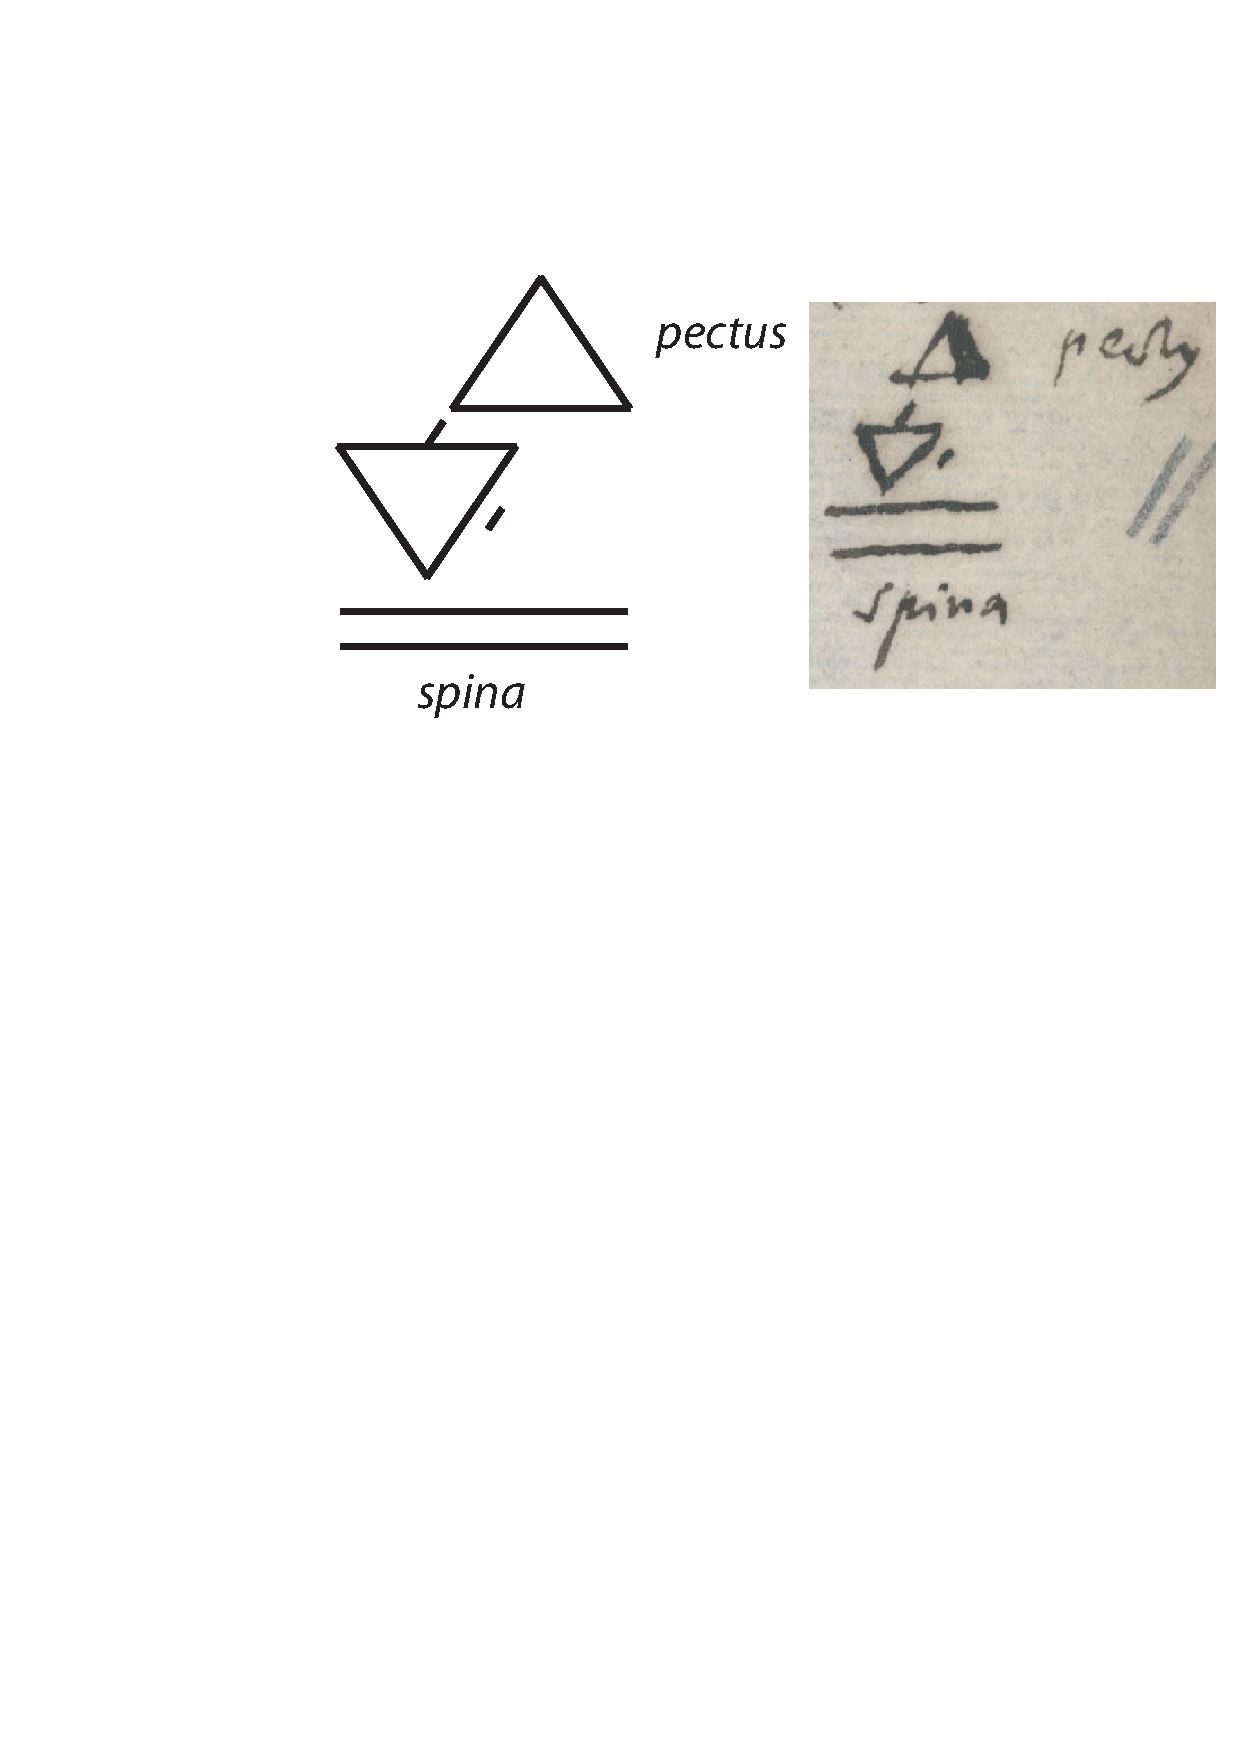
\includegraphics[trim = 0mm -3mm 0mm 0mm, clip, width=0.48\textwidth]{images/lh0040104b_011r1.pdf}\\
%\centering [\textit{Fig. 14}]
%%\end{wrapfigure}%
%\pend
\pstart
\centering
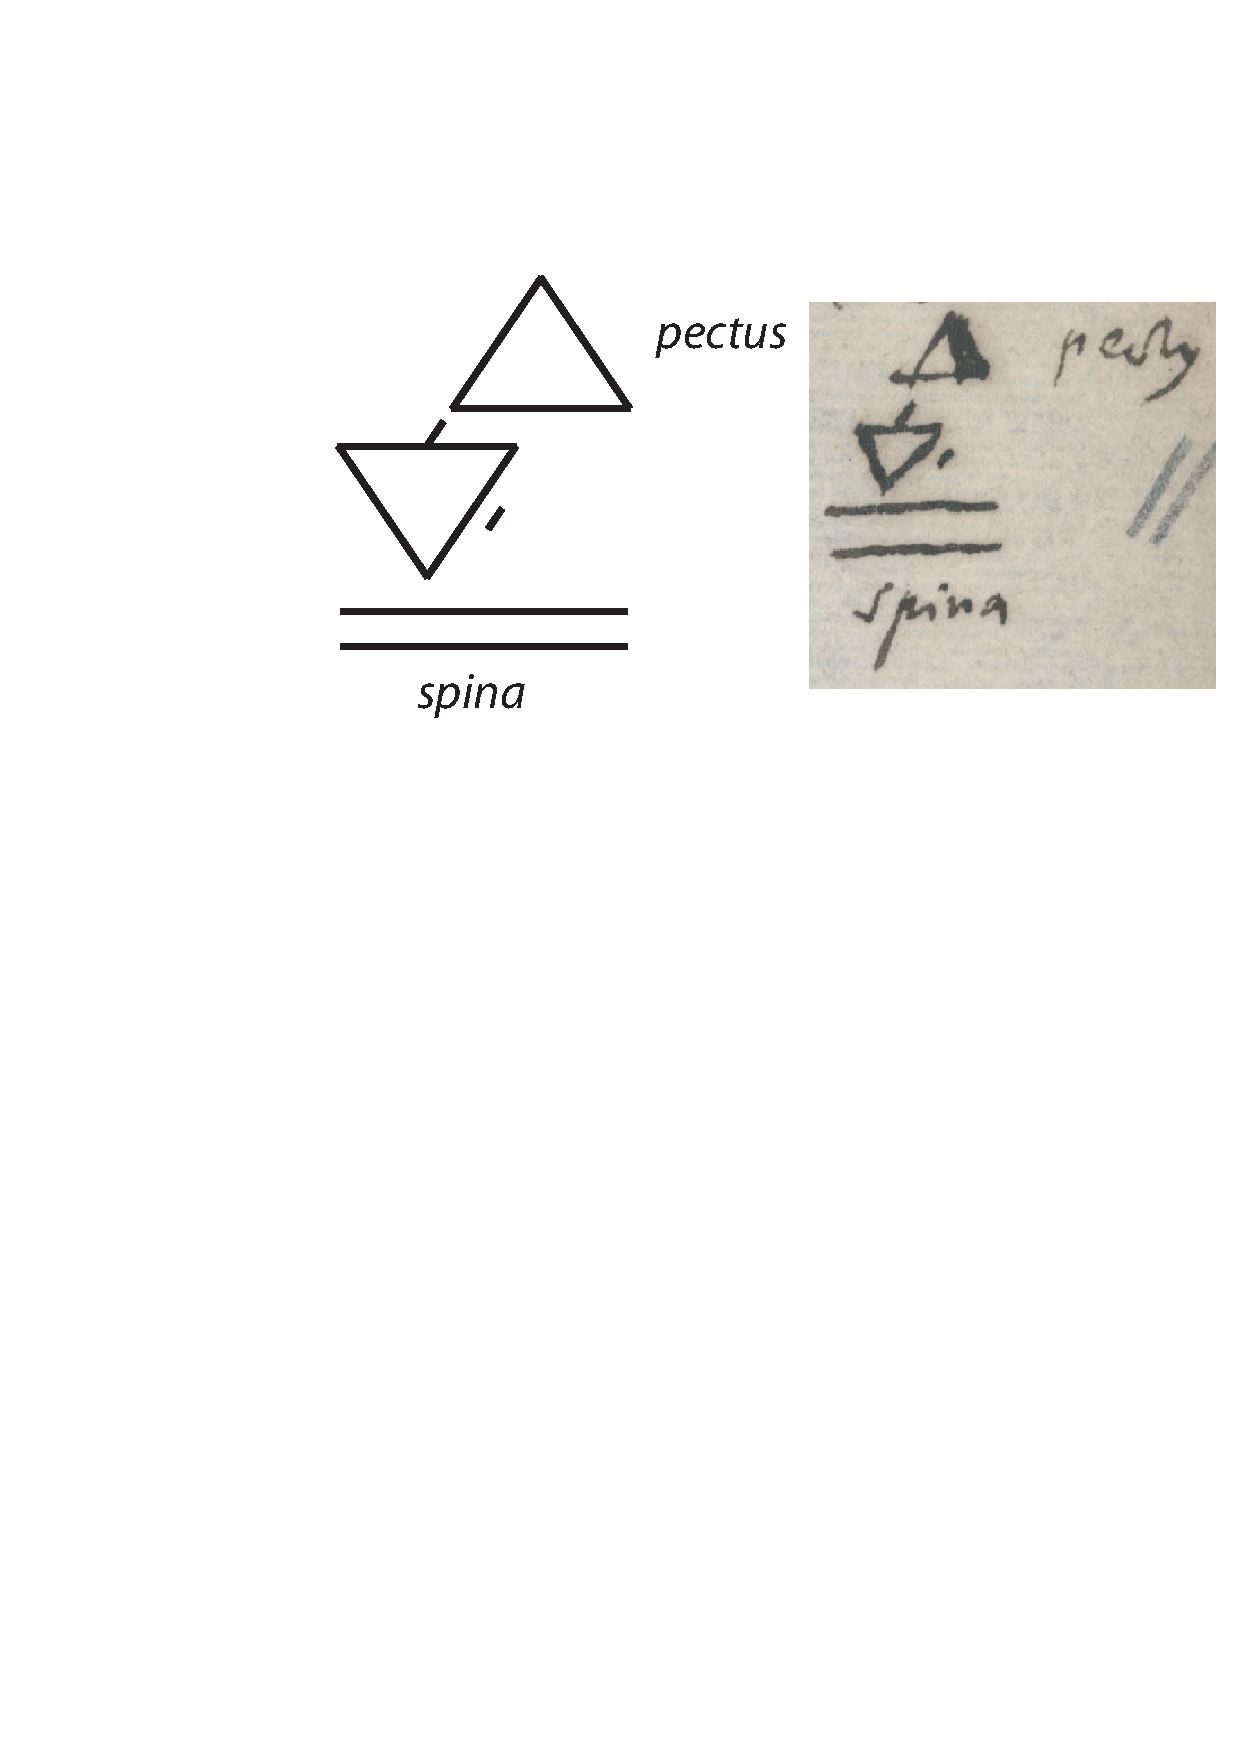
\includegraphics[trim = 0mm -3mm 0mm 0mm, clip, width=0.48\textwidth]{images/lh0040104b_011r1.pdf}\\
\centering [\textit{Fig. 14}]
%\end{wrapfigure}%
\pend
\vspace{1em}
\pstart
%
Vena\setline{1} \edtext{}{\lemma{}\Afootnote{\textit{Am oberen Rand von Bl. 11~r\textsuperscript{o}:} Pars V excerptorum anatomicorum ex Mso. Cartesii\vspace{-4mm}\protect\index{Namensregister}{\textso{Descartes}, René (1596-1650)}}}arteriosa directe per medium pectoris e corde egrediebatur atque ibi erat interstitium duarum ejus valvularum, cum tertia esset duabus arteriae venosae parallela; haecque est a parte anteriore, velut alia a posteriore.
Inter\-jacet autem pars aortae ascendens, et arteria venosa statim versus sinistram, et spinam reflectitur.
\pend
%\newpage
\pstart
Sanguis ex sinistro ventriculo ascendit per unicum orificium
\edtext{[quod]}{\lemma{qui}\Bfootnote{\textit{L \"{a}ndert Hrsg.}}}
statim in alia duo dividitur, anterius et posterius. Anterius est aorta ascendens, posterius deorsum a sinistris reflexum est descendens; eique jungitur ramus ex vena arteriosa.
\pend%
\pstart%
Orificium venae arteriosae per quod sanguis ex dextro ventriculo egreditur est in ipso corde magis versus sinistrum latus quam orificium aortae. His inspectis recte videor conjicere solum primum cordis ventriculum formatum fuisse ante umbilicum, ac tunc inchoata omnia solida membra et excrementa in ore, in vesica, et circa totum corpus collecta.
\pend%
\pstart%
Notavi arterias umbilicales nato foetu sponte contrahi nec manere nisi pelliculam eas integentem, quae in ligamentum abit earumque extremitatem ex contractione claudi. Videtur descendisse oesophagus una cum nervis sexti paris usque ad cordis viciniam priusquam foetus aleretur per umbilicum, ac deinde sanguine adveniente ex umbilico exspumasse unde pulmones, qui postea crescentes nervos recurrentes versus caput reduxerunt; redundasse, unde lien recta versus spinam, et hepar versus pectus; ac viam excremento cerebri abundasse unde ventriculus et ex mora oesophagi in vicinia cordis antequam ventriculus fieret hujus orificium superius. Tunc autem etiam vel formatus vel auctus est dexter cordis ventriculus quod effecit, ut oesophagus inter cavam et truncum \makebox[1.0\textwidth][s]{aortae descendentem transierit, versus latus sinistrum; et dum inflatus est ventriculus}
\pend
\newpage
\pstart\noindent protrusit hepar versus latus dextrum; quod demonstratur ex eo quod in gallinis ubi dexter cordis ventriculus tenuissima tantum pelle tegitur et ventriculus et hepar manent in \edtext{medio corporis:}{\lemma{medio}\Bfootnote{\textit{(1)}\ cordis \textit{(2)}\ corporis: \textit{L}}}
adhaeret autem ventriculus in parte superiore et posteriore, lieni in anteriore hepati, cui communicando aliquas arterias ejus sanguis vicinus exspumavit in bilem unde vesica biliaria, quae adjuncta illi parti ventriculi, effecit ut ibi perforaretur, et producta sunt intestina innumeris modis inflexa prout bilis exitum quaerens volvebatur.
\pend%
\pstart%
Cordis dexter ventriculus videtur eodem fere tempore factus quo sinister, originem enim habet ex eo quod cum materia subtilior sive mobilior in medium cor laberetur, et inde per liniam rectam versus caput ascenderet spumosior et magis aerea circa illam se vertebat, quare vero verteretur a spina versus dextrum latus (ut apparet ex fluxu venae coronariae) potius quam versus sinistrum, est difficultas quam hactenus enodare non potui. Huic dextri cordis ventriculi productioni non obest quod postea umbilicus factus sit accurate in medio ventris, non in parte dextra; nondum enim formato ventriculo truncus aortae, a quo pendebat locus umbilici nihilominus mansit in medio corporis saltem ad sensum, nam quod paulo magis vergeret in sinistrum latus quam in dextrum, patet ex eo quod venam conscendat ex parte sinistra inter emulgentes et ilia hincque etiam fortasse est, quod pars corporis dextra soleat esse robustior quam sinistra quia scilicet est aliquanto carnosior.
\pend%
\pstart%
Formatur autem necessario secundus ventriculus ex eo quod multae sint aeriae particulae in sanguine quae cum non tam cito possent relabi in cor, quam terreae et 
\edtext{[aqueae],}{\lemma{aquae}\Bfootnote{\textit{L \"{a}ndert Hrsg.}}}
facilius autem inflammarentur, ad latus ipsarum, sive in ambitu debuerunt dilatari.
\pend%
\pstart%
 In avibus major est inaequalitas inter dextrum et sinistrum cordis sinum, quam in quadrupedibus quod sero, eorum sanguis minus abundat, adeoque est multo calidior, aereis particulis destitutus, iis vero involutus, minus habet virium.
\pend%
\pstart%
Coctis 6 ovis quibus gallina per 15 dies et amplius incubuerat inveni cum dura cocta essent in omnibus majorem extremitatem solo aere plenam esse. Ac fracta deinde pellicula per quam totam multae venae spargebantur, aliquid aquae elapsum est sicque inter corticem et superiorem ovi partem aliquid spatii intercessit, in omnibus autem foetus erat in superiori parte sinistro lateri incumbens, ita scilicet ut sinistrum latus versus acutiorem ovi partem respiceret, pullusque esset incurvatus, tegebaturque pelle quadam ex albumine facta ex qua etiam plumulae crescere videbantur. Infra pullum erat vitellus, infra vitellum
\edtext{denique}{\lemma{denique}\Bfootnote{\textit{erg. L}}}
erat albumen, quod in quinque ovis corticis exteriori parti firmiter adhaerebat ibique erat durius quam paulo altius, et linea sive cavitate quadam orbiculari a superiori albuminis ovi parte distinguebatur; in sexto tamen ovo nulla talis distinctio erat an forte quia in 5 illis ovis duae chalazae fuerunt, in illo una tantum. Supra albumen erat vitellus, ab eo etiam linea quadam inter utrumque excavata distinctus, sed in ea ovi parte in qua erat dorsum pulli albumen supra vitellum ascendebat, quod videbatur esse ad alendum ejus integumentum in parte autem pulli anteriore inter ejus caput et podicem pars vitelli satis crassa sursum ascendebat, ex qua pendebat umbilicus, et extra corpus pulli, loco umbilici videbantur esse intestina, intus autem non apparuerunt intestina, sed tantum cor valde album, cujus dextra cavitas major quam sinistra et non ita in orbem curvata, ut in adultis videbatur et hepar valde magnum et forsan pulmo, et corpus quoddam valde album, quod pro ventriculo accepi, denique rostri pars superior albidior erat, et incipiebat durescere.
[11~v\textsuperscript{o}]
\pend%
%\count\Bfootins=1500
%\count\Cfootins=1500
%\count\Afootins=1500